\documentclass[12pt,a4paper]{article}

\usepackage[T1]{fontenc}
\usepackage[utf8]{inputenc}
\usepackage{ctex}
\usepackage{amsmath,amsfonts,amssymb,amsthm}
\usepackage{abstract,appendix,natbib,caption}
\usepackage{makeidx,hyperref,url,booktabs}
\usepackage{graphicx,epsfig,subfig}
\usepackage{geometry}
\usepackage{xcolor}

\newtheorem{theorem}{定理}

\geometry{scale=0.8}

%\setlength{\lineskip}{\baselineskip}
\setlength{\parskip}{0.5\baselineskip}

\title{Anderson局部化实验总结}
\author{sis-flag}
\date{\today}

\begin{document}

\maketitle

\begin{abstract}
Anderson局部化是量子力学里面的一个重要问题。这里主要通过实验模拟,研究不同边界条件下 Anderson局部化模型的相关性质。
\end{abstract}

\section{理论说明}

\subsection{问题介绍}

Anderson局部化模型,在数学上表示为特征值问题
\begin{align}
- \triangle u(x) + V(x) u(x) = \lambda u(x) \qquad x \in \Omega
\end{align}
求解区域$\Omega = [0,1]^d$,维数$d = 1, 2$。

一维的情况时,区域$\Omega=[0,1]$被均匀分成$M$个区间,区域$\Omega=[0,1] \times [0,1]$被均匀分成$M \times M$个方格。在每个方格上$V(x)$是分片常数,而且大于等于0。

$V(x)$一般有两种选取方式,一种是取为区间$[0, K]$之内的均匀分布。另一种是在$\{0, K\}$内,以概率$p$取$0$,概率$1-p$取为$K$的二项分布。

方程的边界条件可以是固定边界条件
\begin{align}
- \Delta u(x) + V(x) u(x) = \lambda u(x) \qquad x \in \Omega \\
u(x) = 0 \qquad x \in \partial \Omega
\end{align}
和导数边界条件,参数满足$h \geq 0$,$\mathbf{n}$代表外法向量。
\begin{align}
- \Delta u(x) + V(x) u(x) = \lambda u(x) \qquad x \in \Omega \\
\frac{\partial u}{\partial \mathbf{n}}(x) + h u(x) = 0 \qquad x \in \partial \Omega
\end{align}

\subsection{landscape}

固定边界条件的特征值问题对应方程
\begin{align}
- \Delta w(x) + V(x) w(x) = 1 \qquad x \in \Omega \\
w(x) = 0 \qquad x \in \partial \Omega
\end{align}
导数边界条件的特征值问题对应方程
\begin{align}
- \Delta w(x) + V(x) w(x) = 1 \qquad x \in \Omega \setminus G \\
\frac{\partial u}{\partial \mathbf{n}}(x) = h / \beta \qquad x \in \partial \Omega \\
\end{align}
其中$\beta > 0$是任意常数。

方程的解$w(x)$叫做\textbf{landscape}。

\begin{theorem}

在特征值问题中,特征值$\lambda_k$,对应特征函数$u_k(x)$,满足$\max_{x \in \Omega} |u_k(x)| = 1$。$w_k(x)$是对应的landscape,则

固定边界条件下,它们满足
\begin{align}
|u_k(x)| \leq \lambda_k |w(x)| \qquad x \in \Omega
\end{align}
导数边界条件下,它们满足
\begin{align}
|u_k(x)| \leq (\lambda_k + \beta) |w(x)| \qquad x \in \Omega
\end{align}

\end{theorem}

证明略。

\subsection{共振现象}

\begin{theorem}

在特征值问题中,某个给定的特征值$\lambda^{(\Omega)}$,对应特征函数$u^{(\Omega)}(x)$。子区域$D \subset \Omega$。

固定边界条件下,$\lambda_k^{(D)}$和$u_k^{(D)}(x)$是下面这个问题的特征值和特征函数
\begin{align}
-\triangle u^{(D)}(x) + V(x) u^{(D)}(x) = \lambda^{(D)} u^{(D)}(x) \qquad x \in D \\
u^{(D)}(x) = 0 \qquad x \in \partial D
\end{align}
函数$v(x)$是下面这个问题的解
\begin{align}
-\triangle v(x) + V(x) v(x) = 0 \qquad x \in D \\
v(x) = 0 \qquad x \in \partial D \cap \partial \Omega \\
v(x) = u^{(\Omega)}(x) \qquad x \in \partial D \setminus \partial \Omega
\end{align}

导数边界条件下,$\lambda_k^{(D)}$和$u_k^{(D)}(x)$是下面这个问题的特征值和特征函数
\begin{align}
-\triangle u^{(D)}(x) + V(x) u^{(D)}(x) = \lambda^{(D)} u^{(D)}(x) \qquad x \in D \\
\frac{\partial u^{(D)}}{\partial \mathbf{n}}(x) + h u^{(D)}(x) = 0 \qquad x \in \partial D \cap \partial \Omega \\
u^{(D)}(x) = 0 \qquad x \in \partial D \setminus \partial \Omega
\end{align}
函数$v(x)$是下面这个问题的解
\begin{align}
-\triangle v(x) + V(x) v(x) = 0 \qquad x \in D \\
\frac{\partial v}{\partial \mathbf{n}}(x) + h v(x) = 0 \qquad x \in \partial D \cap \partial \Omega \\
v(x) = u^{(\Omega)}(x) \qquad x \in \partial D \setminus \partial \Omega
\end{align}

则特征函数满足
\begin{align}
\|u^{(\Omega)}\|_{L^2(D)} \leq (1 + \frac{\lambda^{(\Omega)}}{d}) \|v\|_{L^2(D)}
\end{align}
其中$d = \min_k |\lambda^{(\Omega)} - \lambda_k^{(D)}|$

\end{theorem}

\textbf{证明}

定义算子$L = -\triangle + V$,它是一个正的,对称的算子。

对某个特定的特征值$\lambda^{(\Omega)}$和对应的特征函数$u^{(\Omega)}(x)$,在子区域$D$上,假设我们知道$u^{(\Omega)}$在边界$\partial D$上的值,则$u^{(\Omega)}$在内部的值可以看作这样一个方程的解。
\begin{align}
L u - \lambda^{(\Omega)} u = 0 \qquad x \in D \\
\frac{\partial u}{\partial \mathbf{n}} + h u = 0 \qquad x \in \partial D \cap \partial \Omega \\
u = u^{(\Omega)} \qquad x \in \partial D \setminus \partial \Omega
\end{align}

在子区域$D$上,函数$v(x)$满足的边界条件相同。此时$w = u - v$在边界上就是零边界条件。

在子区域$D$上考虑特征值问题
\begin{align}
L u_k^{(D)} = \lambda_k^{(D)} u_k^{(D)}
\end{align}

对应特征函数$u_k^{(D)}$构成整个空间的一组正交的Hilbert基。把$w$按这组基函数展开,得到
\begin{align}
w(x) = \sum_k w_k \ u_k^{(D)}(x) \qquad w_k = \int_{D} w(x) \ u_k^{(D)}(x) \ dx
\end{align}

此时有
\begin{align}
L w = \sum_k \lambda_k^{(D)} w_k u_k^{(D)} \qquad L w - \lambda^{(\Omega)} w = \sum_k (\lambda_k^{(D)} - \lambda^{(\Omega)}) w_k u_k^{(D)}
\end{align}
就得到
\begin{align}\label{eq0}
\| L w - \lambda^{(\Omega)} w \|_{L^2(D)}^2 = \sum_k (\lambda_k^{(D)} - \lambda^{(\Omega)})^2 w_k^2 \geq \min_k (\lambda_k^{(D)} - \lambda^{(\Omega)})^2\sum_k w_k^2 = d^2 \|w\|_{L^2(D)}^2
\end{align}
注意到$L u - \lambda u = 0, L v = 0$,就是$L w - \lambda w = L(u - v) - \lambda(u - v) = \lambda v$。

因此得到
\begin{align}
\lambda^{(\Omega)} \| v \|_{L^2(D)} \geq d \|w\|_{L^2(D)}
\end{align}
就是
\begin{align}
\|u^{(\Omega)}\|_{L^2(D)} \leq \|v\|_{L^2(D)} + \|w\|_{L^2(D)} \leq (1 + \frac{\lambda^{(\Omega)}}{d}) \|v\|_{L^2(D)}
\end{align}
对固定边界条件,证明类似。

证毕。

这个定理解释了“共振”现象。在应用中,我们可以把$D$取成valley line划分出的子区域。这样的子区域边界上$u(x)|_{\partial D}$一般特别小,此时齐次方程的解$v(x)$也很小。如果想要特征函数聚集在这一片区域,也就是$\|u\|_{L^2(D)}$很大的时候,就 只能是$d$很小。这说明,\textbf{如果一块valley line划分出的区域上,特征值和当前特征值很接近,那么特征函数就会聚集到这一片子区域里。}

\subsection{特征函数的下界}

\begin{theorem}

在特征值问题中,某个给定的特征值$\lambda^{(\Omega)}$,对应特征函数$u^{(\Omega)}(x)$。$\lambda_k^{(D)}$和$v(x)$定义同上。$\lambda_1^{(D)} = \min_k \lambda_k^{(D)}$。
则特征函数满足
\begin{align}
\|u^{(\Omega)}\|_{L^2(D)} \geq \frac{\lambda_1^{(D)}}{\lambda^{(\Omega)} + \lambda_1^{(D)}} \|v\|_{L^2(D)}
\end{align}

\end{theorem}

\textbf{证明}

直接把上面的证明中,公式\ref{eq0}改成
\begin{align}
\|L w\|_{L^2(D)}^2 = \sum_k (\lambda_k^{(D)})^2 w_k^2 \geq (\lambda_1^{(D)})^2 \sum_k w_k^2 = (\lambda_1^{(D)})^2 \|w\|_{L^2(D)}^2
\end{align}
注意到$L u - \lambda u = 0, L v = 0$,就是$L w = - \lambda u$。得到
\begin{align}
\lambda^{(\Omega)} \|u\|_{L^2(D)} \geq \lambda_1^{(D)} \|u - v\|_{L^2(D)}
\end{align}
也就是
\begin{align}
(\lambda^{(\Omega)} + \lambda_1^{(D)}) \|u\|_{L^2(D)} \geq \lambda_1^{(D)} (\|u - v\|_{L^2(D)} + \|u\|_{L^2(D)}) \geq \lambda_1^{(D)} \|v\|_{L^2(D)}
\end{align}

证毕。

目前还没想出它有什么物理意义。

把$D$取成$\Omega_{\epsilon} = \{x \in \Omega : dist(x, \partial \Omega) > \epsilon\}$,再让$\epsilon$趋于0。极限状态下,$\lambda_k^{(D)} = \lambda_k^{(\Omega)}$。此时函数$v(x)$是下面这个问题的解
\begin{align}
-\triangle v(x) + V(x) v(x) = 0 \qquad x \in \Omega \\
v(x) = u^{(\Omega)}(x) \qquad x \in \partial \Omega
\end{align}

不等式变为
\begin{align}
\|u_k\|_{L^2(\Omega)} \geq \frac{\lambda_1^{(\Omega)}}{\lambda_k^{(\Omega)} + \lambda_1^{(\Omega)}} \|v_k\|_{L^2(\Omega)}
\end{align}

对于最小特征值$k=1$的情况,就是
\begin{align}
\|u_k\|_{L^2(\Omega)} \geq \frac12 \|v_k\|_{L^2(\Omega)}
\end{align}
最小特征函数的下界是同样边界条件下调和函数的一半。

目前也没想出它有什么物理意义。。。

\subsection{K很大时的极限性态}

\begin{theorem}

定义$D = \{x \in \Omega | V(x) = 0 \}$,$D^C$就是势函数非零的部分。对问题的特征函数(归一化到最大值为1),满足

\begin{align}
\lim_{K \rightarrow \infty} u(x) = 0 \qquad x \in D^C
\end{align}

\end{theorem}

证明略。

这个定理说明,在K很大的情况下,在势函数非0的地方,特征函数会趋近于0。

根据之前共振的结论,我们可以把共振的子区域$D$选为$V(x) > 0$的某个连通子区域。考虑子区域上的特征值问题
\begin{align}
-\Delta u = \lambda u \qquad \mathbf{x} \in D \\
\frac{\partial u}{\partial n} + h u = 0 \qquad \mathbf{x} \in \partial D \cap \partial \Omega \\
u = 0 \qquad \mathbf{x} \in \partial D \setminus \partial \Omega
\end{align}
如果子区域上的特征值和大区域上的特征值相近,就说明特征函数会localize到这一块子区域。

因此,要判断最小的几个特征值localize到哪片区域,就转化成了\textbf{哪片区域上,拉普拉斯方程的特征值最小?}这样的问题。

\subsection{数值模拟方法}

我们使用谱元法而不是通常的有限元或者有限差分方法来计算特征函数。谱元法用分片勒让德多项式作为基底逼近方程的精确解,同时限制数值解整体连续。和通常差分方法的误差收敛阶为$\mathcal{O}(h^{-2})$不同,谱元法在这样的问题上可以达到指数收敛,收敛阶为$\mathcal{O}(e^{-N})$。谱元法的计算量只有$\mathcal{O}(M^2 N^2)$,这使得谱元法可以轻易计算大规模的问题。最后,谱元法中的高次多项式可以很好地刻画问题特征函数的奇异性,从而达到更高的精度。本文中我们选择分片10次多项式模拟所有问题。

翻译:

Eigenmodes are simulated by spectrum elment method instead of ordinary finite element or finite difference method. Legendre polynomials are used in the spectral element method as basis to approximate the solution, while enforce the overall continuty. Ordinary FDM or FEM can only get second-order convergence $\mathcal{O}(h^{-2})$, but the spectral element method can achieve expontial convergence $\mathcal{O}(e^{-N})$ on this problem. Matrix size in spectrual elment method is $\mathcal{O}(M^2 N^2)$, which make it possible for us to simulate large-scale problems. What's more, high degree polynomials can charaterize the singularity of eigenmodes, which can help us attain more accuracy. In this paper, we use picewise polynomial with degree 10 to simulate the following problems.

\section{valley line 相关实验}\label{valley}

\subsection{valley line 和 effective valley line}

valley line 是在landscape函数的基础上,画出函数值较小的部分。这些线把区域划分成了很多小块。根据landscape的控制原理,我们可以确定,这些线可以大致把特征值聚集的区域分割开。由于只有在$w(x) < 1/(\lambda_k + \beta)$的时候,valley line 才真正起到作用。因此我们可以只画出满足条件的线,也就是effective valley line。

我们通过均匀分布生成势函数,在Neumann边界条件下模拟问题。图\ref{VL1}中画出了对应的势函数和landscape和valley line。图\ref{VL2}中画出了一些特征函数和它们对应的effective valley line。

\begin{figure}[htbp]
\centering
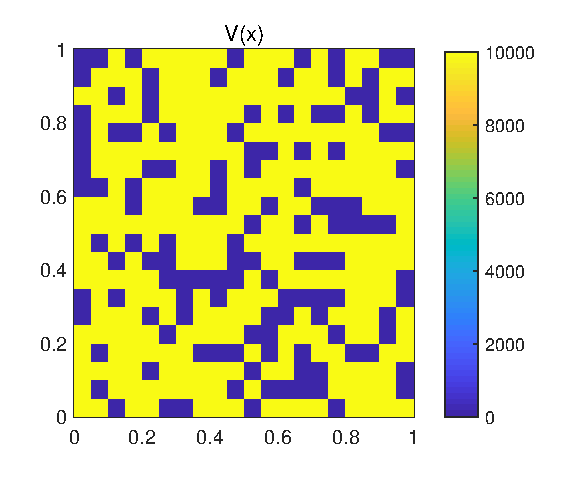
\includegraphics[width=0.3\linewidth]{valley/V}
\includegraphics[width=0.3\linewidth]{valley/W}
\caption{势函数和landscape}
\label{VL1}
\end{figure}

\begin{figure}[htbp]
\centering
\includegraphics[width=0.3\linewidth]{valley/U(1)}
\includegraphics[width=0.3\linewidth]{valley/U(2)}
\includegraphics[width=0.3\linewidth]{valley/U(3)}
\includegraphics[width=0.3\linewidth]{valley/U(5)}
\includegraphics[width=0.3\linewidth]{valley/U(7)}
\includegraphics[width=0.3\linewidth]{valley/U(10)}
\includegraphics[width=0.3\linewidth]{valley/U(20)}
\includegraphics[width=0.3\linewidth]{valley/U(30)}
\includegraphics[width=0.3\linewidth]{valley/U(50)}
\caption{特征函数和effective valley line}
\label{VL2}
\end{figure}

可以看出,在Neumann边界条件下,effective valley line对特征函数的控制也是很好的。

\subsection{子区域划分}

对于landscape,我们也可以这样看:找到一个阈值,将landscape大于这个阈值的子区域找出来,研究该子区域的分块情况。我们把$w(x) < 1/(\lambda_k + \beta)$的区域涂蓝,其它区域涂黄。在相同的参数下,把划分出的子区域和特征函数进行对比,结果如图\ref{BL}。

\begin{figure}[htbp]
\centering
\includegraphics[width=0.4\linewidth]{valley/B(1)}
\includegraphics[width=0.4\linewidth]{valley/B(2)}
\includegraphics[width=0.4\linewidth]{valley/B(3)}
\includegraphics[width=0.4\linewidth]{valley/B(5)}
\includegraphics[width=0.4\linewidth]{valley/B(7)}
\includegraphics[width=0.4\linewidth]{valley/B(10)}
\includegraphics[width=0.4\linewidth]{valley/B(20)}
\includegraphics[width=0.4\linewidth]{valley/B(30)}
\caption{特征函数和子区域划分}
\label{BL}
\end{figure}

虽然有点难看,但是可以看出,特征函数聚集的位置确实在蓝色的区域内部。

\newpage

\section{边界条件的影响}\label{boundary}

\subsection{验证边界条件的影响}

仿照PNAS文章里的参数,取K为8000,V取均匀分布。生成一维和二维的势函数如图\ref{bd-V}。在这个势函数下,分别在不同边界下模拟问题。
\begin{figure}[htbp]
\centering
\includegraphics[width=0.3\linewidth]{boundary/V1d}
\includegraphics[width=0.3\linewidth]{boundary/V2d}
\caption{势函数}
\label{bd-V}
\end{figure}

一维情况下,分别在不同边界条件下模拟问题,得到图\ref{bd-1d}。图中Robin边界条件中取$h=1, \beta=30$。Neumann边界条件中取$\beta=0$。图中黑色的线代表landscape,彩色的线表示不同特征值下的$u_k(x) / (\lambda_k + \beta)$。
\begin{figure}[htbp]
\centering
\includegraphics[width=0.3\linewidth]{boundary/D1d}
\includegraphics[width=0.3\linewidth]{boundary/N1d}
\includegraphics[width=0.3\linewidth]{boundary/R1d}
\caption{一维模拟结果}
\label{bd-1d}
\end{figure}

可以看出,landscape能很好地控制特征函数。在一维情况下,不同的边界条件主要影响landscape,对聚集在区间内部的特征值影响很小。

一维情况下,分别在不同边界条件下模拟问题,得到图\ref{bd-2d}。边界条件和参数相同。
\begin{figure}[htbp]
\centering
\includegraphics[width=0.4\linewidth]{boundary/Dw2d}
\includegraphics[width=0.4\linewidth]{boundary/Du2d}
\includegraphics[width=0.4\linewidth]{boundary/Nw2d}
\includegraphics[width=0.4\linewidth]{boundary/Nu2d}
\includegraphics[width=0.4\linewidth]{boundary/Rw2d}
\includegraphics[width=0.4\linewidth]{boundary/Ru2d}
\caption{二维模拟结果}
\label{bd-2d}
\end{figure}

可以看出,在二维的情况下,不同边界条件对解和特征函数有很大影响。固定边界条件的峰一定会出现在区域内部,而导数边界条件下的峰会出现在区域边界。

\subsection{边界条件对landscape的影响}

在实验中我们发现,边界条件主要影响landscape的边界,对landscape的内部影响较小。对eigenmode的影响就比较大,原来不会聚集到边界的峰有可能聚集到边界了。在这里我们详细说明一下这种现象。

还是先看一维的情况,势函数和前面的例子相同。把不同边界条件下的landscape画在一起,如图\ref{bdc-1d}

\begin{figure}[htbp]
\centering
\includegraphics[width=0.3\linewidth]{boundary/C1d}
\caption{不同边界条件下的landscape}
\label{bdc-1d}
\end{figure}

可以看出,landscape在内部几乎相同,只有边界上不一样。这说明边界条件主要影响landscape的边界部分。

二维情况也类似。由于二维的曲面画在一起不容易看清楚,我们画出切面图。如图\ref{bdc-2d}。
\begin{figure}[htbp]
\centering
\includegraphics[width=0.3\linewidth]{boundary/C2d(0)}
\includegraphics[width=0.3\linewidth]{boundary/C2d(1)}
\includegraphics[width=0.3\linewidth]{boundary/C2d(2)}
\includegraphics[width=0.3\linewidth]{boundary/C2d(3)}
\includegraphics[width=0.3\linewidth]{boundary/C2d(4)}
\includegraphics[width=0.3\linewidth]{boundary/C2d(5)}
\caption{二维不同边界条件下的landscape}
\label{bdc-2d}
\end{figure}

可以看出,二维的情况也支持前面的结论。\textbf{不同的边界条件只影响边界附近的landscape。landscape在内部几乎相同,只有边界上不一样。}

\subsection{边界条件对eigenmode的影响}

我们希望知道不同边界条件下会不会对特征函数产生影响。我们还是先看一维的情况。在图\ref{be1}中我们比较了不同边界条件下的特征函数。

\begin{figure}[htbp]
\centering
\includegraphics[width=0.24\linewidth]{boundary/V1}
\includegraphics[width=0.24\linewidth]{boundary/E1(1)}
\includegraphics[width=0.24\linewidth]{boundary/E1(2)}
\includegraphics[width=0.24\linewidth]{boundary/E1(3)}
\includegraphics[width=0.24\linewidth]{boundary/E1(5)}
\includegraphics[width=0.24\linewidth]{boundary/E1(7)}
\includegraphics[width=0.24\linewidth]{boundary/E1(10)}
\includegraphics[width=0.24\linewidth]{boundary/E1(20)}
\caption{不同边界条件下eignemode的比较(右上第一张为势函数V)}
\label{be1}
\end{figure}

这里得到的结论和我们的直觉相反,对前几个特征值,两种边界条件下的结果都一样,但是对后面的特征值,两种边界条件下就表现出了很大差异。注意到这个例子中没有前几个特征值localize到边界的情况,我们尝试模拟一下前面提到过的特殊选取,让特征函数出现在边界。结果如图\ref{be2}。

\begin{figure}[htbp]
\centering
\includegraphics[width=0.24\linewidth]{boundary/V2}
\includegraphics[width=0.24\linewidth]{boundary/E2(1)}
\includegraphics[width=0.24\linewidth]{boundary/E2(2)}
\includegraphics[width=0.24\linewidth]{boundary/E2(3)}
\includegraphics[width=0.24\linewidth]{boundary/E2(5)}
\includegraphics[width=0.24\linewidth]{boundary/E2(7)}
\includegraphics[width=0.24\linewidth]{boundary/E2(10)}
\includegraphics[width=0.24\linewidth]{boundary/E2(20)}
\caption{不同边界条件下eignemode的比较(右上第一张为势函数V)}
\label{be2}
\end{figure}

可以看到,除了eigenmode3,其它的都有很大差异。

下面我们研究二维的情况。模拟结果如图\ref{be3}由于二维的情况大多数都localize在边界,所以两种边界条件下的情况完全不一样。如果eigenmode在边界附近出现了峰,那不同的边界条件就会对它影响很大。

\begin{figure}[htbp]
\centering
\includegraphics[width=0.3\linewidth]{boundary/V3} \\
\includegraphics[width=0.4\linewidth]{boundary/E3(1)}
\includegraphics[width=0.4\linewidth]{boundary/E3(2)}
\includegraphics[width=0.4\linewidth]{boundary/E3(5)}
\includegraphics[width=0.4\linewidth]{boundary/E3(7)}
\includegraphics[width=0.4\linewidth]{boundary/E3(10)}
\includegraphics[width=0.4\linewidth]{boundary/E3(20)}
\caption{不同边界条件下eignemode的比较}
\label{be3}
\end{figure}

所以我们的结论还是和前面提到的一样:\textbf{边界条件只影响边界。所以localize到内部的eigenmode不会有影响,只影响localize到边界的特征函数。}

\subsection{边界条件对特征值的影响}

在这里,一维和二维的例子有很大的区别。在前面的三个例子中,画出两种不同边界下的特征值如图\ref{be4}。图中横轴为特征值编号(第几小的特征值),纵轴为特征值的数值。

\begin{figure}[htbp]
\centering
\includegraphics[width=0.3\linewidth]{boundary/lam1}
\includegraphics[width=0.3\linewidth]{boundary/lam2}
\includegraphics[width=0.3\linewidth]{boundary/lam3}
\caption{不同边界条件下特征值的数值}
\label{be4}
\end{figure}

可以看出,一维情况下,两种边界条件下对应排序的特征值相差很小,但是二维的时候就相差很大。((这个也可以验证特征值增长的阶)。从实验可以看出,\textbf{一维情况下,边界条件对特征值几乎没有影响,二维情况下,边界条件对特征值和特征函数的影响十分显著。}

\newpage

\section{势函数的影响}\label{potential}

在取Bernoulli分布时,二维情形$p$有临界值0.59。$p$大于这个临界值时,$V(x)=0$的子区域应该是连成一片的;小于这个临界值时,$V(x)=0$的子区域应该分成很多小块。选取不同的参数$p$,画出二维势函数的图像如图\ref{p0}。图中可以清晰地看出区域连成一片的现象。

\begin{figure}[htbp]
\centering
\includegraphics[width=0.3\linewidth]{potential/P3V}
\includegraphics[width=0.3\linewidth]{potential/P5V}
\includegraphics[width=0.3\linewidth]{potential/P7V}
\caption{不同概率生成的势函数}
\label{p0}
\end{figure}

\subsection{均匀分布的势函数}

$V(x)$由均匀分布生成,选取不同的K,在Neumann边界条件下模拟问题。得到结果如图\ref{P0}。

\begin{figure}[htbp]
\centering
\includegraphics[width=0.4\linewidth]{potential/P0V} \\
\includegraphics[width=0.4\linewidth]{potential/P0K1W}
\includegraphics[width=0.4\linewidth]{potential/P0K1U}
\includegraphics[width=0.4\linewidth]{potential/P0K2W}
\includegraphics[width=0.4\linewidth]{potential/P0K2U}
\includegraphics[width=0.4\linewidth]{potential/P0K3W}
\includegraphics[width=0.4\linewidth]{potential/P0K3U}
\includegraphics[width=0.4\linewidth]{potential/P0K4W}
\includegraphics[width=0.4\linewidth]{potential/P0K4U}
\caption{均匀分布模拟结果}
\label{P0}
\end{figure}

可以看出,随着K趋于无穷,landscape和特征函数会逐渐聚集到势函数最小的一片区域内。

\subsection{Bernoulli分布的势函数}

$V(x)$由Bernoulli分布生成,选取不同的K和p,在Neumann边界条件下模拟问题。得到结果如图\ref{P3},图\ref{P5}和图\ref{P7}。

\begin{figure}[htbp]
\centering
\includegraphics[width=0.4\linewidth]{potential/P3V} \\
\includegraphics[width=0.4\linewidth]{potential/P3K1W}
\includegraphics[width=0.4\linewidth]{potential/P3K1U}
\includegraphics[width=0.4\linewidth]{potential/P3K2W}
\includegraphics[width=0.4\linewidth]{potential/P3K2U}
\includegraphics[width=0.4\linewidth]{potential/P3K3W}
\includegraphics[width=0.4\linewidth]{potential/P3K3U}
\includegraphics[width=0.4\linewidth]{potential/P3K4W}
\includegraphics[width=0.4\linewidth]{potential/P3K4U}
\caption{p=0.3 模拟结果}
\label{P3}
\end{figure}

\begin{figure}[htbp]
\centering
\includegraphics[width=0.4\linewidth]{potential/P5V} \\
\includegraphics[width=0.4\linewidth]{potential/P5K1W}
\includegraphics[width=0.4\linewidth]{potential/P5K1U}
\includegraphics[width=0.4\linewidth]{potential/P5K2W}
\includegraphics[width=0.4\linewidth]{potential/P5K2U}
\includegraphics[width=0.4\linewidth]{potential/P5K3W}
\includegraphics[width=0.4\linewidth]{potential/P5K3U}
\includegraphics[width=0.4\linewidth]{potential/P5K4W}
\includegraphics[width=0.4\linewidth]{potential/P5K4U}
\caption{p=0.5 模拟结果}
\label{P5}
\end{figure}

\begin{figure}[htbp]
\centering
\includegraphics[width=0.4\linewidth]{potential/P7V} \\
\includegraphics[width=0.4\linewidth]{potential/P7K1W}
\includegraphics[width=0.4\linewidth]{potential/P7K1U}
\includegraphics[width=0.4\linewidth]{potential/P7K2W}
\includegraphics[width=0.4\linewidth]{potential/P7K2U}
\includegraphics[width=0.4\linewidth]{potential/P7K3W}
\includegraphics[width=0.4\linewidth]{potential/P7K3U}
\includegraphics[width=0.4\linewidth]{potential/P7K4W}
\includegraphics[width=0.4\linewidth]{potential/P7K4U}
\caption{p=0.7 模拟结果}
\label{P7}
\end{figure}

从图中可以看出,在K趋于无穷时,landscape和特征函数在$V(x) = K$的部分内会趋于0。即使是在p比较大的时候,$V(x)=0$子区域已经连成一片,这个结论依然正确。这可以很好地验证我们的理论。

此外我们通过比较均匀分布和Bernoulli分布下的landscape可以看出,在均匀分布下,随着K的增大,landscape会逐渐趋于0,而在Bernoulli分布下,landscape不会趋于0。

\newpage

\section{最优参数的选取}\label{parameter}

%\subsection{$\alpha$的选取}
%
%注意到,如果已知方程
%\begin{align}
%- \Delta w(x) + V(x) w(x) = 1 \qquad x \in \Omega \\
%\frac{\partial u}{\partial \mathbf{n}}(x) = h / \beta \qquad x \in \partial \Omega \\
%\end{align}
%在$x_0$处,解的函数值为$w_0$,那它也可以看成方程
%\begin{align}
%- \Delta w(x) + V(x) w(x) = 1 \qquad x \in \Omega \\
%\frac{\partial u}{\partial \mathbf{n}}(x) = h / \beta \qquad x \in \partial \Omega \\
%w(x_0) = w_0 \qquad x = w_0
%\end{align}
%的解。因此,我们可以直接求解没有固定边界的方程,此时$1/\alpha$可以在$w(x)$的最大值和最小值之间任意选择。由于我们想要达到最优的控制条件,$\alpha$一般选取为$w(x)$最大值的倒数。
%
%我们先从一维的简单情况开始。选取$K = 8000$,Neumann边界条件。分别选取$x_0 = 0.3, 0.5, 0.7$。 对不同的$\alpha$模拟,由于问题是Neumann边界条件,可以直接选取$\beta = 0$。结果如图\ref{A1}和图\ref{A2}。图中的黑色线是landscape,彩色的线是特征函数$u_k(x) / (\lambda_k + \alpha + \beta)$。
%
%\begin{figure}[htbp]
%\centering
%\includegraphics[width=0.3\linewidth]{parameter/W1X3A1000}
%\includegraphics[width=0.3\linewidth]{parameter/W1X3A3000}
%\includegraphics[width=0.3\linewidth]{parameter/W1X3A10000}
%\includegraphics[width=0.3\linewidth]{parameter/W1X5A1000}
%\includegraphics[width=0.3\linewidth]{parameter/W1X5A3000}
%\includegraphics[width=0.3\linewidth]{parameter/W1X5A10000}
%\includegraphics[width=0.3\linewidth]{parameter/W1X7A1000}
%\includegraphics[width=0.3\linewidth]{parameter/W1X7A3000}
%\includegraphics[width=0.3\linewidth]{parameter/W1X7A10000}
%\caption{均匀分布模拟结果}
%\label{A1}
%\end{figure}
%
%\begin{figure}[htbp]
%\centering
%\includegraphics[width=0.3\linewidth]{parameter/W2X3A1000}
%\includegraphics[width=0.3\linewidth]{parameter/W2X3A3000}
%\includegraphics[width=0.3\linewidth]{parameter/W2X3A10000}
%\includegraphics[width=0.3\linewidth]{parameter/W2X5A1000}
%\includegraphics[width=0.3\linewidth]{parameter/W2X5A3000}
%\includegraphics[width=0.3\linewidth]{parameter/W2X5A10000}
%\includegraphics[width=0.3\linewidth]{parameter/W2X7A1000}
%\includegraphics[width=0.3\linewidth]{parameter/W2X7A3000}
%\includegraphics[width=0.3\linewidth]{parameter/W2X7A10000}
%\caption{Bernoulli分布模拟结果}
%\label{A2}
%\end{figure}
%
%从图中可以看出,似乎是$\alpha$越小越好。而且更重要的一个现象是:\textbf{不同的$\alpha$选取仅仅改变landscape在$x_0$附近的性态,对其它位置的没什么变化。}为了验证这个现象,我们把两次实验中所有的9条landscape画在一起。如图\ref{ALLA}。
%\begin{figure}[htbp]
%\centering
%\includegraphics[width=0.3\linewidth]{parameter/ALL1}
%\includegraphics[width=0.3\linewidth]{parameter/ALL2}
%\caption{两种分布下的所有landscape}
%\label{ALLA}
%\end{figure}
%
%根据理论,固定$\alpha$,$u_k(x) / (\lambda_k + \alpha + \beta) \leq w(x)$。应该对任意的$x_0$都成立,然而不等式的右边没有出现$x_0$。那就是说
%\begin{align}
%u_k(x) / (\lambda_k + \alpha + \beta) \leq \inf_{x_0 \in \Omega} w(x)
%\end{align}
%根据实验结果,$\alpha$的选取只影响$x_0$附近的函数性态,因此,改变不同的$x_0$时,landscape应该很靠近no-enforce下的landscape,因此我们在误差允许的情况下,近似可以看作
%\begin{align}
%u_k(x) / (\lambda_k + \alpha + \beta) \leq \inf_{x_0 \in \Omega} w(x) \approx w_{\text{no-enforce}} (x)
%\end{align}
%也就是
%\begin{align}
%u_k(x) / (\lambda_k + \alpha + \beta) \leq \approx w_{\text{no-enforce}} (x) \qquad \forall \alpha > 0
%\end{align}
%注意到不等号右边,没有$\alpha$,于是可以得出,在误差允许范围内
%\begin{align}
%u_k(x) / (\lambda_k + \beta) \leq \approx w_{\text{no-enforce}} (x)
%\end{align}
%\textbf{可以直接把$\alpha$扔掉。}
%
%为了验证这个现象,我们取$\alpha=200$,在不同的$x_0$下画出landscape(彩色的线),并且和no-enforce的(黑色的线)进行比较。可以看出,图中各种彩色的线下界和黑色的线很像,说明这样近似是合理的。如图\ref{INF}。
%\begin{figure}[htbp]
%\centering
%\includegraphics[width=0.3\linewidth]{parameter/INF1}
%\includegraphics[width=0.3\linewidth]{parameter/INF2}
%\caption{所有landscape}
%\label{INF}
%\end{figure}
%
%在二维情况,这种现象特别明显,$\alpha$的影响范围远远小于一维的情况,如图\ref{2DA}。
%\begin{figure}[htbp]
%\centering
%\includegraphics[width=0.3\linewidth]{parameter/2DA1}
%\includegraphics[width=0.3\linewidth]{parameter/2DA2}
%\caption{两种landscape对比图}
%\label{2DA}
%\end{figure}
%
%综合以上现象,$\alpha$可以直接扔掉。

\subsection{$\beta$的选取}

还是首先在一维情况下实验,Robin边界条件,取$K = 8000, h=10$,其他参数同上,实验结果如图\ref{B3}和\ref{B4}。根据之前的实验(图\ref{bdc-1d}),$\beta$主要改变landscape在边界上的部分,对内部的影响不大。

\begin{figure}[htbp]
\centering
\includegraphics[width=0.3\linewidth]{parameter/W3B100}
\includegraphics[width=0.3\linewidth]{parameter/W3B1000}
\includegraphics[width=0.3\linewidth]{parameter/W3B10000}
\caption{均匀分布模拟结果}
\label{B3}
\end{figure}

\begin{figure}[htbp]
\centering
\includegraphics[width=0.3\linewidth]{parameter/W4B100}
\includegraphics[width=0.3\linewidth]{parameter/W4B1000}
\includegraphics[width=0.3\linewidth]{parameter/W4B10000}
\caption{Bernoulli分布模拟结果}
\label{B4}
\end{figure}

从图中可以看出,$\beta$不能太小,否则边界会翘起来,也不能太大,否则不等式就不精确了。

对于什么样的参数是“最优”,并没有统一的标准。这里我们选取的标准是landscape和特征函数之间的gap$\|w - u_k/(lam_k + \beta)\|_{L^2} / \|w\|_{L^2}$。选取不同的$\beta$,画出gap随$\beta$变化的趋势。结果如图\ref{BG}。图中不同颜色的线代表不同的$k$。
\begin{figure}[htbp]
\centering
\includegraphics[width=0.3\linewidth]{parameter/gap3}
\includegraphics[width=0.3\linewidth]{parameter/gap4}
\caption{模拟结果}
\label{BG}
\end{figure}

从图中可以看出,对于均匀分布,最优的$\beta$大概在300左右,而对于Bernoulli分布,$\beta$似乎是越小越好。

\newpage

\section{峰值位置定位}\label{locate}

这里我们研究K很大,且V为伯努利分布的情况。

对于一维的情况。一维长度为$l$的区间上,Dirichlet边界条件的特征值为$\lambda = \frac{\pi^2}{l^2}, \frac{4 \pi^2}{l^2}, \frac{9 \pi^2}{l^2}, \cdots $。所以想要判断问题localize的区域和特征值大小,只要表示出每个区域上的特征值,然后排序就可以了。

对于原问题为Neumann边界条件的情况,一维长度为$l$的区间上,一半Dirichlet边界一半Neumann边界条件的特征值为$\lambda = \frac{\pi^2}{4 l^2}, \frac{9 \pi^2}{4 l^2}, \frac{25 \pi^2}{4 l^2}, \cdots $。其它部分和Dirichlet边界一样。

因此,主要解决的是二维或者更高维的情况。{\color{red} 二维的情况下,子区域未必是单连通的。}下面我们分别在Dirichlet边界条件和Neumann边界条件下实验这个问题。下面的图\ref{V}中画出了测试用的势函数$V(x)$,
\begin{figure}[htbp]
\centering
\includegraphics[width=0.4\linewidth]{locate/V}
\caption{势函数}
\label{V}
\end{figure}

\textbf{Dirichlet边界}

首先我们要确保K足够大。我们分别选取$K_1=1.0 \times 10^7$和$K_2=1.1 \times 10^7$模拟问题。表\ref{kD}中列出了在两个参数下特征函数的差别(特征函数归一化到$\max u = 1$)。可以看出,此时继续增大$K$的值,特征函数和特征值变化也不会很大。

\begin{table}
\centering
\begin{tabular}{c|c|c|c}
\hline
特征值序号 & $\max |u_1 - u_2|$ & $|\lambda_1 - \lambda_2|$ & $|\lambda_1 - \lambda_2| / \lambda_2$ \\
\hline
1 & 1.92e-03 & 1.317 & 7.40e-04 \\
2 & 1.82e-03 & 1.309 & 7.33e-04 \\
3 & 3.50e-03 & 3.909 & 1.37e-03 \\
4 & 3.83e-03 & 3.853 & 1.32e-03 \\
5 & 3.45e-03 & 3.982 & 1.34e-03 \\
6 & 3.23e-03 & 3.919 & 1.23e-03 \\
7 & 3.13e-03 & 3.869 & 1.20e-03 \\
8 & 3.21e-03 & 3.831 & 1.17e-03 \\
9 & 3.10e-03 & 3.692 & 1.08e-03 \\
\hline 
\end{tabular}
\caption{验证K足够大}
\label{kD}
\end{table}

我们猜想,Dirichlet边界下,一块区域上最小的特征值和这块区域的(面积/周长)成正比。为了验证这个猜想,我们把区域内所有除了$1\times1$和$1\times2$的子区域都找出来编号,如图\ref{rD}。(这里工作量貌似不大,编号是用人力完成的)

\begin{figure}[htbp]
\centering
\includegraphics[width=0.4\linewidth]{locate/edVD}
\caption{区域编号(Dirichlet边界)}
\label{rD}
\end{figure}

图\ref{eD}中画出了最小的9个特征函数。可以看出,第1,2,3,4,7,9个特征函数,都对应着子区域上的最小特征函数。第5,6个对应区域上第二小的特征函数。第8个对应子区域上第三小的特征函数。

\begin{figure}[htbp]
\centering
\includegraphics[width=0.3\linewidth]{locate/eigD1}
\includegraphics[width=0.3\linewidth]{locate/eigD2}
\includegraphics[width=0.3\linewidth]{locate/eigD3}
\includegraphics[width=0.3\linewidth]{locate/eigD4}
\includegraphics[width=0.3\linewidth]{locate/eigD5}
\includegraphics[width=0.3\linewidth]{locate/eigD6}
\includegraphics[width=0.3\linewidth]{locate/eigD7}
\includegraphics[width=0.3\linewidth]{locate/eigD8}
\includegraphics[width=0.3\linewidth]{locate/eigD9}
\caption{Dirichlet边界特征函数}
\label{eD}
\end{figure}

这里需要指出的是:某个区域上,第一个特征值比另一个区域小,其它特征值未必也比另一个区域小。从实验中可以看出,8号区域的第一个特征值比7号和12号都大,但是3号区域上的第二个特征值就比其它区域都小了。所以说,如果有某项近似准则能够判断特征值localize到哪一片区域,也\textbf{只是对特征函数是单峰的情况适用}。

表\ref{tD}中列出了这些区域的周长和面积等信息,可以看出,(面积/周长)确实是一个描述相对趋势的指标,但是这个指标不够精确。4号区域的(面积/周长)很大,但是前9个特征值没有一个聚集在她里面。8号区域看起来形状很奇怪,但是(面积/周长)反而最大。12号区域和10号区域面积和周长完全一样,特征值却相差很大。

\begin{table}
\centering
\begin{tabular}{c|c|c|c|c|c|c}
\hline
编号 & 面积 & 周长 & 面积/周长 & (面积/周长)排名 & 聚集在此处的单峰特征值 & 特征值排名 \\
\hline
8 & 14 & 24 & 0.583 & 1 & 2856 & 3 \\
7 & 7 & 14 & 0.5 & 2 & 1786 & 2 \\
10 & 10 & 20 & 0.5 & 3 & 2968 & 5 \\
12 & 7 & 14 & 0.5 & 4 & 1780 & 1 \\
4 & 6 & 14 & 0.429 & 5 & / & / \\
3 & 4 & 10 & 0.4 & 6 & 3219 & 7 \\
6 & 4 & 10 & 0.4 & 7 & / & / \\
1 & 3 & 8 & 0.375 & 8 & / & / \\
2 & 3 & 8 & 0.375 & 9 & / & / \\
5 & 3 & 8 & 0.375 & 10 & / & / \\
9 & 3 & 8 & 0.375 & 11 & / & / \\
11 & 3 & 8 & 0.375 & 12 & / & / \\
\hline 
\end{tabular}
\caption{Dirichlet边界区域统计}
\label{tD}
\end{table}

综上所述,我们还需要找到一些更有效的指标来刻画它。

\textbf{Neumann边界}

首先我们要确保K足够大。选取同样的参数实验,结果见表\ref{kN}。

\begin{table}
\centering
\begin{tabular}{c|c|c|c}
\hline
特征值序号 & $\max |u_1 - u_2|$ & $|\lambda_1 - \lambda_2|$ & $|\lambda_1 - \lambda_2| / \lambda_2$ \\
\hline
1 & 1.56e-03 & 0.402 & 5.42e-04 \\
2 & 1.07e-03 & 0.678 & 6.05e-04 \\
3 & 4.93e-04 & 0.694 & 5.67e-04 \\
4 & 4.93e-04 & 0.830 & 5.34e-04 \\
5 & 1.92e-03 & 1.317 & 7.40e-04 \\
6 & 1.82e-03 & 1.309 & 7.33e-04 \\
7 & 4.93e-04 & 1.233 & 6.29e-04 \\
8 & 4.93e-04 & 1.233 & 6.29e-04 \\
9 & 4.93e-04 & 1.233 & 6.29e-04 \\
\hline 
\end{tabular}
\caption{验证K足够大}
\label{kN}
\end{table}

对于Neumann边界,我们注意到边界上的对称性。在一维的情况下,一半是Neumann边界一半是Dirichlet边界的区域上,最小的特征值,可以看成把区域进行偶延拓,在两倍长的区域上求解Dirichlet边界的特征值。如图\ref{expand}。因此,我们如果要比较特征值,需要比较子区域沿边界延拓出去之后的新区域上的特征值。\textbf{这个方法就可以解释,为什么对Neumann边界条件,特征函数更容易聚集在边界附近。}

\begin{figure}[htbp]
\centering
\includegraphics[height=0.15\textheight]{locate/DN}
\includegraphics[height=0.15\textheight]{locate/DD}
\caption{混合边界特征函数的延拓}
\label{expand}
\end{figure}

注意,这个延拓只对最小的特征值成立,对第二小的特征值就不成立了。

基于这种猜想,我们把区域内所有除了$1\times1$和$1\times2$在内部的子区域和除了$1\times1$在边界上的子区域都找出来编号,如图\ref{rN}。(这里编号也是用人力完成的)

\begin{figure}[htbp]
\centering
\includegraphics[width=0.4\linewidth]{locate/edVN}
\caption{区域编号(Neumann边界)}
\label{rN}
\end{figure}

同样的势函数$V(x)$下,边界条件为Neumann边界条件。图\ref{eN}中画出了最小的9个特征函数。可以看出,除了第4个特征函数,其它都对应着子区域上的最小特征函数。

\begin{figure}[htbp]
\centering
\includegraphics[width=0.3\linewidth]{locate/eigN1}
\includegraphics[width=0.3\linewidth]{locate/eigN2}
\includegraphics[width=0.3\linewidth]{locate/eigN3}
\includegraphics[width=0.3\linewidth]{locate/eigN4}
\includegraphics[width=0.3\linewidth]{locate/eigN5}
\includegraphics[width=0.3\linewidth]{locate/eigN6}
\includegraphics[width=0.3\linewidth]{locate/eigN7}
\includegraphics[width=0.3\linewidth]{locate/eigN8}
\includegraphics[width=0.3\linewidth]{locate/eigN9}
\caption{Neumann边界特征函数}
\label{eN}
\end{figure}

表\ref{tN}中列出了这些区域的周长和面积等信息。这次效果略好,至少前三个预测对了。第7,8,9,10个特征值也预测对了。

\begin{table}
\centering
\begin{tabular}{c|c|c|c|c|c|c}
\hline
编号 & 面积 & 周长 & 面积/周长 & (面积/周长)排名 & 聚集在此处的单峰特征值 & 特征值排名 \\
\hline
1 & 12 & 16 & 0.75 & 1 & 741 & 1 \\
4 & 12 & 18 & 0.666 & 2 & 1120 & 2 \\
14 & 8 & 12 & 0.666 & 3 & 1225 & 3 \\
8 & 14 & 24 & 0.583 & 4 & / & / \\
7 & 7 & 14 & 0.5 & 5 & 1786 & 6 \\
10 & 10 & 20 & 0.5 & 6 & / & / \\
12 & 7 & 14 & 0.5 & 7 & 1780 & 5 \\
16 & 4 & 8 & 0.5 & 8 & / & / \\
17 & 4 & 8 & 0.5 & 9 & 1959 & 7 \\
18 & 4 & 8 & 0.5 & 10 & 1959 & 9 \\
19 & 4 & 8 & 0.5 & 11 & 1959 & 8 \\
3 & 4 & 10 & 0.4 & 12 & / & / \\
6 & 4 & 10 & 0.4 & 13 & / & / \\
13 & 4 & 10 & 0.4 & 14 & / & / \\
15 & 4 & 10 & 0.4 & 15 & / & / \\
2 & 3 & 8 & 0.375 & 16 & / & / \\
5 & 3 & 8 & 0.375 & 17 & / & / \\
9 & 3 & 8 & 0.375 & 18 & / & / \\
11 & 3 & 8 & 0.375 & 19 & / & / \\
\hline 
\end{tabular}
\caption{Neumann边界区域统计}
\label{tN}
\end{table}

观察到,在不同边界条件下,localize到相同区域的两个特征值是一样的。这可以验证前面的共振理论。

还可以观察到,Neumann边界条件下,16,17,18,19号区域对应的特征值都近似相等,这也可以验证共振的理论。

综上所述,我们还需要找到一些更有效的指标来刻画它。

\textbf{Robin边界:目前还没有办法}

\textbf{结论}
\begin{itemize}
\item K很大时,局部化问题转化成每个子区域上的拉普拉斯特征值问题。
\item 可以用偶延拓的方法把混合Neumann边界的子问题转化为Dirichlet边界的子问题。
\item (面积/周长)这个指标不够准确,我们还要寻找其它指标。
\end{itemize}

\end{document}